
\subsection{Scaling Options}

\begin{pgfplotskey}{width=\marg{dimen}}
Sets the width of the final picture to \marg{dimen}. If no |height| is specified, scaling will respect aspect ratios.

\paragraph{Remarks:} 
\begin{itemize}
	\item The scaling only affects the width of one unit in $x$-direction or the height for one unit in $y$-direction. Axis labels and tick labels won't be resized, but their size is used to determine the axis scaling.

	\item You can use the |scale=|\marg{number} option,
\begin{codeexample}[code only]
\begin{tikzpicture}[scale=2]
\begin{axis}
...
\end{axis}
\end{tikzpicture}
\end{codeexample}
	to scale the complete picture.

	\item The \Tikz-options |x| and |y| which set the unit dimensions in $x$ and $y$ directions can be specified as arguments to |\begin{axis}[x=1.5cm,y=2cm]| if needed (see below). These settings override the |width| and |height| options.

	\item You can also force a fixed width/height of the axis (without looking at labels) with
\begin{codeexample}[code only]
\begin{tikzpicture}
\begin{axis}[width=5cm,scale only axis]
	...
\end{axis}
\end{tikzpicture}
\end{codeexample}

	\item Please note that up to the writing of this manual, \PGFPlots\ only estimates the size needed for axis- and tick labels. It does not include legends which have been placed outside of the axis\footnote{I.e. the `\texttt{width}' option will not work as expected, but the bounding box is still ok.}. This may be fixed in future versions.

	Use the |x=|\marg{dimension}, |y=|\marg{dimension} and |scale only axis| options if the scaling happens to be wrong.
\end{itemize}
\end{pgfplotskey}

\begin{pgfplotskey}{height=\marg{dimen}}
	See |width|.
\end{pgfplotskey}

\begin{pgfplotskey}{scale only axis=\mchoice{true,false} (initially false)}
If |scale only axis| is enabled, label, tick and legend dimensions won't influence the size of the axis rectangle, that means |width| and |height| apply only to the axis rectangle

If |scale only axis=false| (the default), \PGFPlots\ will try to produce the desired width \emph{including} labels, titles and ticks.
\end{pgfplotskey}

\begin{pgfplotsxykeylist}{
	\x=\marg{dimen},
	\x={\{(\meta{x},\meta{y})\}}}
Sets the unit vectors for $x$ (or $y$). Every logical plot coordinate $(x,y)$ is drawn at the position
\[ x \cdot \begin{bmatrix} e_{xx} \\ e_{xy} \end{bmatrix} + y \cdot \begin{bmatrix} e_{yx} \\ e_{yy} \end{bmatrix}. \]
The unit vectors $e_x$ and $e_y$ determine the paper position in the current (always two dimensional) image.

The key |x=|\marg{dimen} simply sets $e_x = (\meta{dimen},0)^T $ while |y=|\marg{dimen} sets $e_y = (0,\meta{dimen})^T$.
Here, \marg{dimen} is any \TeX\ size like |1mm|, |2cm| or |5pt|. Note that you should not use a negative \marg{dimen} (consider using |x dir| and its variants to reverse axis directions).
\begin{codeexample}[]
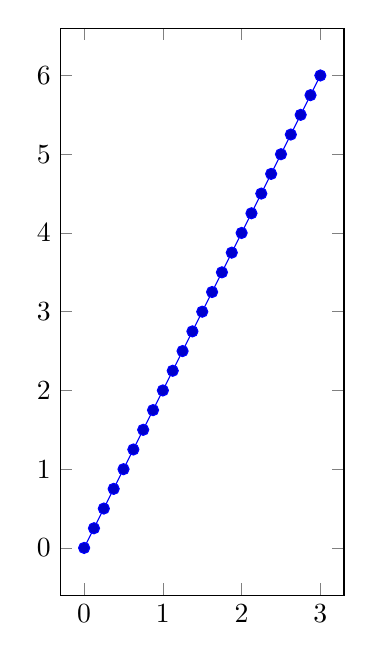
\begin{tikzpicture}
\begin{axis}[x=1cm,y=1cm]
\addplot expression[domain=0:3] {2*x};
\end{axis}
\end{tikzpicture}
\end{codeexample}

\begin{codeexample}[]
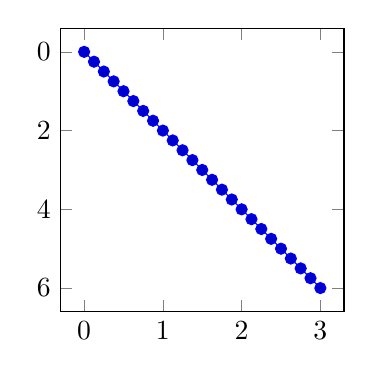
\begin{tikzpicture}
\begin{axis}[x=1cm,y=-0.5cm]
\addplot expression[domain=0:3] {2*x};
\end{axis}
\end{tikzpicture}
\end{codeexample}

The second syntax, |x={(|\meta{x}|,|\meta{y}|)}| sets $e_x = (\meta{x},\meta{y})^T$ explicitly\footnote{Please note that you need extra curly braces around the vector. Otherwise, the comma will be interpreted as separator for the next key-value pair.}; the corresponding |y| key works similarly. This allows to define skewed or rotated axes.

\begin{codeexample}[]
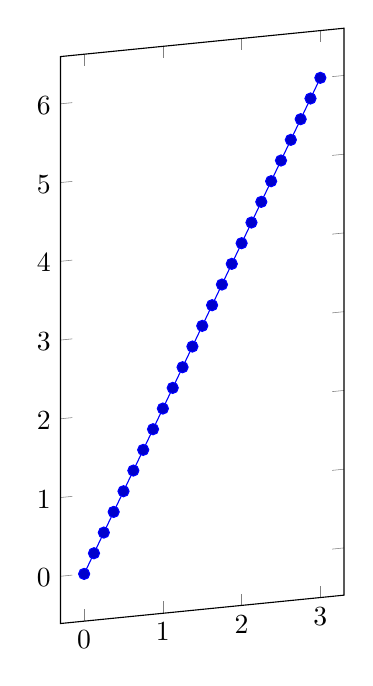
\begin{tikzpicture}
\begin{axis}[x={(1cm,0.1cm)},y=1cm]
\addplot expression[domain=0:3] {2*x};
\end{axis}
\end{tikzpicture}
\end{codeexample}

\begin{codeexample}[]
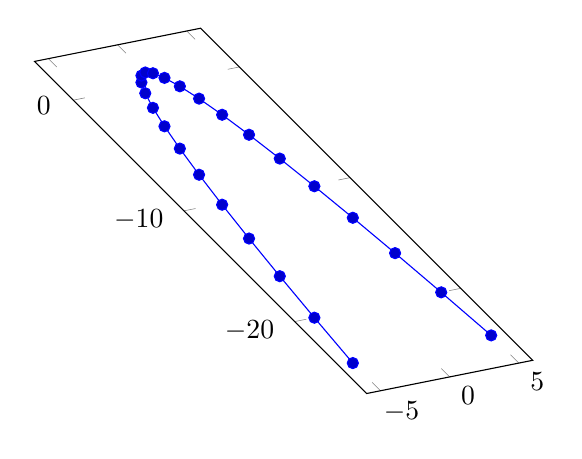
\begin{tikzpicture}
\begin{axis}[
		x={(5pt,1pt)},
		y={(-4pt,4pt)}]
\addplot {1-x^2};
\end{axis}
\end{tikzpicture}
\end{codeexample}

	Setting $x$ explicitly overrides the |width| option. Setting $y$ explicitly overrides the |height| option.

	Setting |x| and/or |y| for logarithmic axis will set the dimension used for $1 \cdot e \approx 2.71828$.

	Please note that it is \emph{not} possible to specify |x| as argument to |tikzpicture|. The option 
\begin{codeexample}[code only]
\begin{tikzpicture}[x=1.5cm]
\begin{axis}
	...
\end{axis}
\end{tikzpicture}
\end{codeexample}
	won't have any effect because an axis rescales its coordinates (see the |width| option).

\begin{codeexample}[]
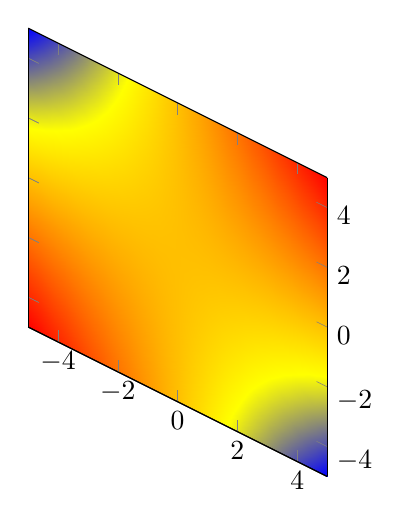
\begin{tikzpicture}
\begin{axis}[
	x={(1cm,-0.5cm)},
	y=1cm,
	z=0cm,
	axis on top,
	scale mode=scale uniformly,
	]
	\addplot3[surf,shader=interp] {x*y};
\end{axis}
\end{tikzpicture}
\end{codeexample}

\paragraph{Explicit units for 3D axes:} As of version~1.5, it is also possible to supply unit vectors to three--dimensional axes. In this case, the following extra assumptions need to be satisfied:
\begin{enumerate}
	\item If you want to control three--dimensional units, you need to provide \emph{all} of |x|, |y|, and |z| keys. For two--dimensional axes, it is also supported to supply just one of |x| or |y|.
	\item Any provided three--dimensional unit vectors are assumed to form a \emph{right--handed coordinate system}. In other words: take you right hand, let the thumb point into the |x| direction, the first finger in |y| direction and the second finger in |z| direction. If that is impossible, the \PGFPlots\ output will be wrong. The reason for this assumption is that \PGFPlots\ needs to compute the view direction out of the provided units (see below).

	Consider using |x dir=reverse| or its variants in case you want to reverse directions.

	\item For a three--dimensional axis, \PGFPlots\ computes a view direction out of the provided unit vectors. The view direction is required to realize the |z buffer| feature (i.e.\ to decide about depths)\footnote{\PGFPlots\ provides a debug option called \texttt{view dir=\marg{x}\marg{y}\marg{z}} to override the view direction, should that ever be interesting.}.
\end{enumerate}
This feature is used to realize the \verbpdfref{\addplot3 graphics} feature, compare the examples in section~\ref{sec:plotgraphics3d} on page~\pageref{sec:plotgraphics3d}.

\paragraph{Limitations:} Unfortunately, skewed axes are \textbf{not available for bar plots}.
\index{Errors!Skewed axes and bar plots}%
\index{Bar Plots!Skewed axes problems}%
\end{pgfplotsxykeylist}

\begin{pgfplotskey}{scale mode=\mchoice{auto,none,stretch to fill,scale uniformly} (initially auto)}
	Specifies how |width|, |height|, and the three unit vector keys |x|, |y|, and |z| are combined to produce the final image.

	The initial choice \declaretext{auto} chooses one of the other possible choices depending on the actual context. More precisely, it is the same as |none| if at least one of |x|, |y|, or |z| is provided (meaning that these keys are the final unit size). If no unit is provided, it defaults to |stretch to fill|.

	The choice |none| does not apply any re-scaling at all. Use this if prescribed lengths of |x|, |y| (and perhaps |z|) should be used. In other words: it ignores |width| and |height|.

	The choice |stretch to fill| takes |x|, |y|, and |z| as they have been found (either from user input or from some automatic processing) and rescales the axis with two \emph{separate} scales: one which results in the proper |width| and one which results in the proper |height|. As a consequence, the unit vectors are modified and distorted such that the final image fits into the prescribed dimensions. This is usually what one expects unless one provides unit directions explicitly.
	
	The choice |scale uniformly| is similar -- but it applies only \emph{one} scaling factor to fit into the prescribed dimensions. This scaling factor will be the same for both, |width| and |height|. Naturally, this will result in unsatisfactory results because either the final width or the final height will not be met. Therefor, this choice will enlarge or shrink limits to get the desired dimensions. Thus, the unit vectors have exactly the same size \emph{relations and angles} as they had before the scaling; only their magnitude is changed uniformly. But due to the given constraints, parts of the image may be empty or may no longer be visible. In case the outcome needs manual improvements, you can improve the visibility by modifying |width| and/or |height| (more freedom is not supported for this choice). Note that \PGFPlots\ implements this rescaling \textbf{if and only if} $e_{yx} = 0$ (for two--dimensional axes) or $e_{zx} = 0$ (for three--dimensional axes). In other words: for two--dimensional axes, the |y| vector has to be parallel to the canvas $y$ direction and for three--dimensional axes, the same holds for the |z| vector. The idea is to rescale only the vertical part of one unit vector and to change the limits of that respective axis simultaneously. The |scale uniformly| choice is used to realize the \verbpdfref{\addplot3 graphics} feature, see the documentation in section~\ref{sec:plotgraphics3d} on page~\pageref{sec:plotgraphics3d} for its examples.

\end{pgfplotskey}

\begin{pgfplotsxykey}{\x mode=\mchoice{normal,linear,log} (initially normal)}
	Allows to choose between linear (=normal) or logarithmic axis scaling or logplots for each $x,y,z$-combination.

	Logarithmic plots use the current setting of |log basis x| and its variants to determine the basis (default is $e$).
	% FIXME : replicated in pgfplots.reference.specifyrange.tex
\end{pgfplotsxykey}

{\def\pgfmanualpdflabel#1#2{}
\begin{pgfplotsxykey}{\x\ dir=\mchoice{normal,reverse} (initially normal)}
	Allows to revert axis directions such that values are given in decreasing order.

	This key is documented in all detail on page~\pageref{key:pgfplots:xydir}.
\end{pgfplotsxykey}
}

\begin{pgfplotskey}{axis equal=\marg{true,false} (initially false)}
	Each unit vector is set to the same length while the axis dimensions stay constant. Afterwards, the size ratios for each unit in $x$ and $y$ will be the same.
	
	Axis limits will be enlarge to compensate for the scaling effect.
\begin{codeexample}[]
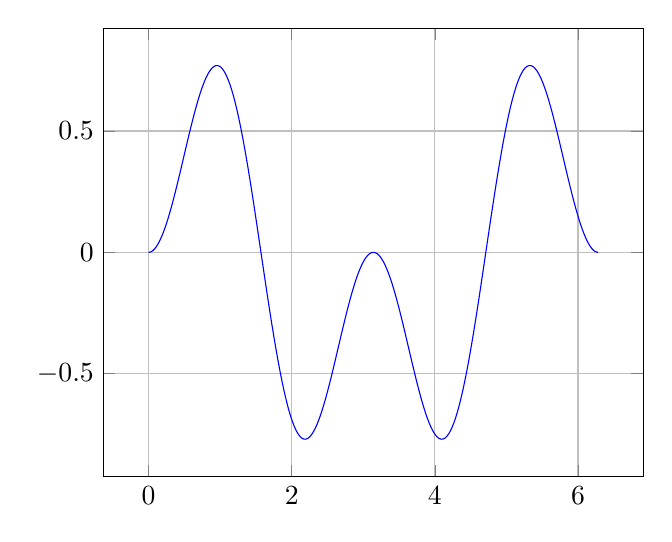
\begin{tikzpicture}
	\begin{axis}[axis equal=false,grid=major]
		\addplot[blue] expression[domain=0:2*pi,samples=300] {sin(deg(x))*sin(2*deg(x))};
	\end{axis}
\end{tikzpicture}
\hspace{1cm}
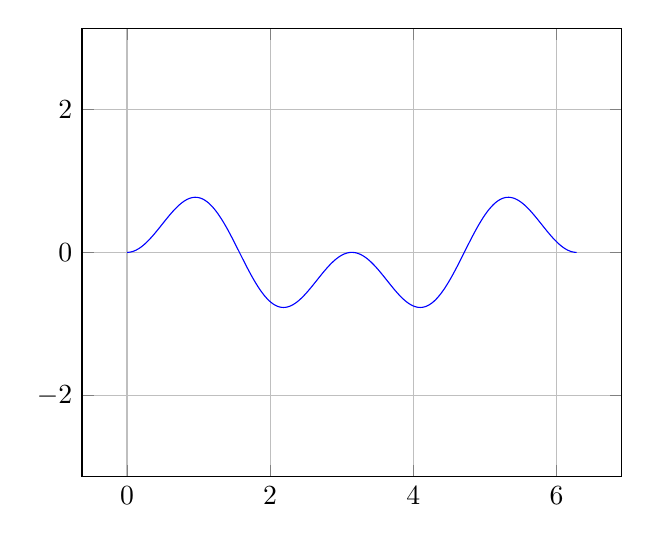
\begin{tikzpicture}
	\begin{axis}[axis equal=true,grid=major]
		\addplot[blue] expression[domain=0:2*pi,samples=300] {sin(deg(x))*sin(2*deg(x))};
	\end{axis}
\end{tikzpicture}
\end{codeexample}
	
\begin{codeexample}[]
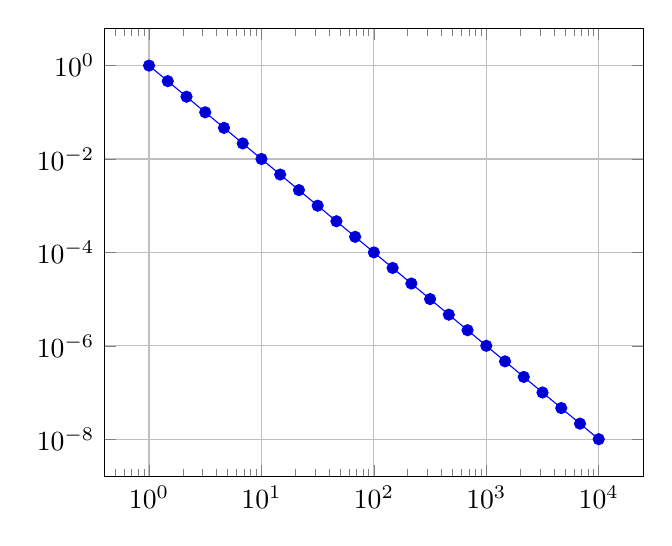
\begin{tikzpicture}
	\begin{loglogaxis}[axis equal=false,grid=major]
		\addplot expression[domain=1:10000] {x^-2};
	\end{loglogaxis}
\end{tikzpicture}
\hspace{1cm}
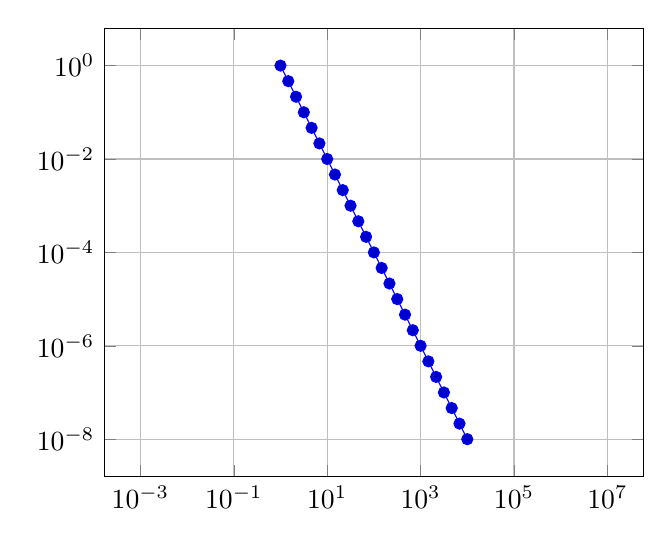
\begin{tikzpicture}
	\begin{loglogaxis}[axis equal=true,grid=major]
		\addplot expression[domain=1:10000] {x^-2};
	\end{loglogaxis}
\end{tikzpicture}
\end{codeexample}
\end{pgfplotskey}

\begin{pgfplotskey}{axis equal image=\marg{true,false} (initially false)}
	Similar to |axis equal|, but the axis limits will stay constant as well (leading to smaller images).
\begin{codeexample}[]
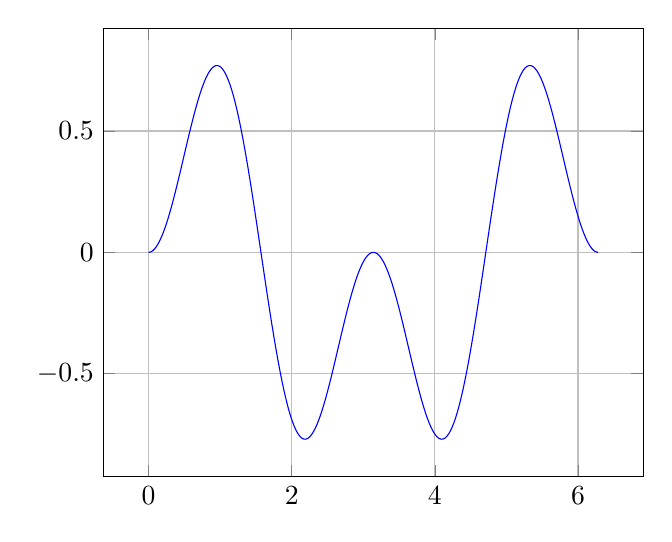
\begin{tikzpicture}
	\begin{axis}[axis equal image=false,grid=major]
		\addplot[blue] expression[domain=0:2*pi,samples=300] {sin(deg(x))*sin(2*deg(x))};
	\end{axis}
\end{tikzpicture}
\hspace{1cm}
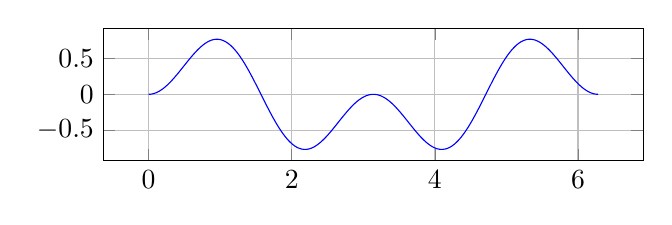
\begin{tikzpicture}
	\begin{axis}[axis equal image=true,grid=major]
		\addplot[blue] expression[domain=0:2*pi,samples=300] {sin(deg(x))*sin(2*deg(x))};
	\end{axis}
\end{tikzpicture}
\end{codeexample}
	
\begin{codeexample}[]
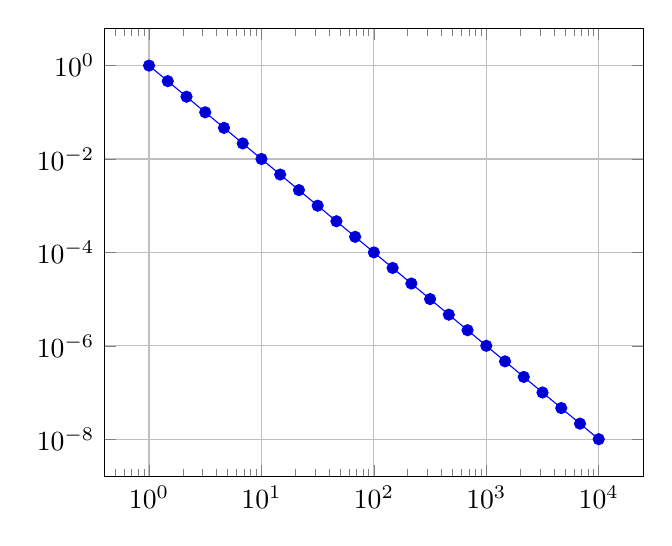
\begin{tikzpicture}
	\begin{loglogaxis}[axis equal image=false,grid=major]
		\addplot expression[domain=1:10000] {x^-2};
	\end{loglogaxis}
\end{tikzpicture}
\hspace{1cm}
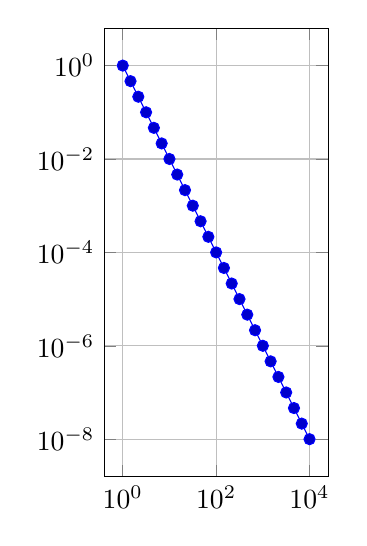
\begin{tikzpicture}
	\begin{loglogaxis}[axis equal image=true,grid=major]
		\addplot expression[domain=1:10000] {x^-2};
	\end{loglogaxis}
\end{tikzpicture}
\end{codeexample}
\end{pgfplotskey}

\begin{pgfplotskey}{unit vector ration=\marg{rx ry rz} (initially empty)}
	Allows to provide custom unit vector ratios. 

	The key allows to tell \PGFPlots\ that, for example, one unit in $x$ direction should be twice as long as one unit in $y$ direction:
\begin{codeexample}[]
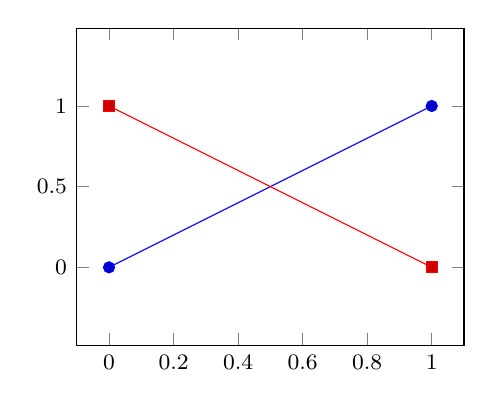
\begin{tikzpicture}
	\begin{axis}[unit vector ratio=2 1,small]
		\addplot coordinates {(0,0) (1,1)};
		\addplot table[row sep=\\,col sep=&] {
			x & y \\
			0 & 1 \\
			1 & 0 \\
		};
	\end{axis}
\end{tikzpicture}
\end{codeexample}
	\noindent Providing |unit vector ratio=2 1| means that $\frac{||e_x||}{||e_y||} = 2$ where each coordinate $(x,y)$ is placed at $x e_x + y e_y \in \R^2$ (see the documentation for |x| and |y| options). Note that |axis equal| is nothing but |unit vector ratio=1 1 1|.

	The arguments \meta{rx}, \meta{ry}, and \meta{rz} are ratios for $x$, $y$ and $z$ vectors, respectively. For two--dimensional axes, only \meta{rx} and \meta{ry} are considered; they are provided relative to the $y$ axis. In other words: the $x$ unit vector will be \meta{rx} $/$ \meta{ry} times longer than the $y$ unit vector. For three--dimensional axes, all three arguments can be provided; they are interpreted relative to the $z$ unit vector. Thus, a three dimensional axis with |unit vector ratio=1 2 4| will have an $x$ unit which is $\nicefrac 14$ the length of the $z$ unit, and a $y$ unit which is $\nicefrac24$ the length of the $z$ unit. 
	
	Trailing values of |1| can be omitted, i.e.\ |unit vector ratio=2 1| is the same as |unit vector ratio=2|; and |unit vector ratio=3 2 1| is the same as |unit vector ratio=3 2|.
	An empty value |unit vector ratio={}| disables unit vector rescaling.

	\begin{pgfplotskeylist}{%
		unit vector ratio*=\marg{rx ry rz},
		unit rescale keep size=\marg{true,false} (initially true)}
	In the default configuration, \PGFPlots\ maintains the original axis dimensions even though |unit vector ratio| involves different scalings. 

	It does so by enlargeing the limits.
\begin{codeexample}[]
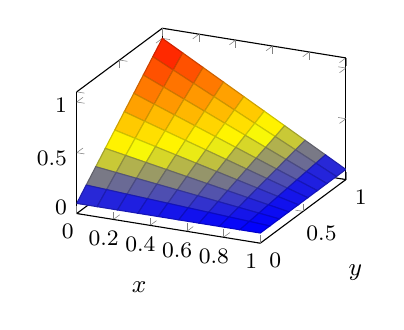
\begin{tikzpicture}
	\begin{axis}[footnotesize,xlabel=$x$,ylabel=$y$,unit vector ratio=]
	\addplot3[surf,samples=10,domain=0:1] {(1-x)*y};
	\end{axis}
\end{tikzpicture}
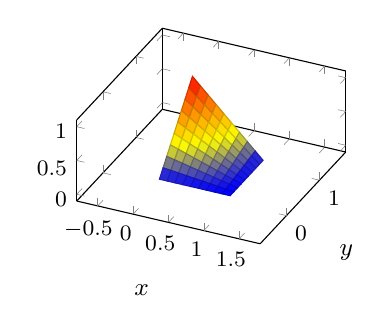
\begin{tikzpicture}
	\begin{axis}[footnotesize,xlabel=$x$,ylabel=$y$,unit vector ratio=1 1 1]
	\addplot3[surf,samples=10,domain=0:1] {(1-x)*y};
	\end{axis}
\end{tikzpicture}
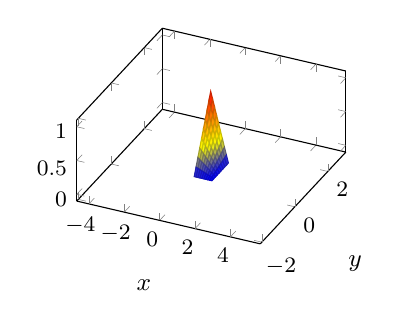
\begin{tikzpicture}
	\begin{axis}[footnotesize,xlabel=$x$,ylabel=$y$,unit vector ratio=0.25 0.5]
	\addplot3[surf,samples=10,domain=0:1] {(1-x)*y};
	\end{axis}
\end{tikzpicture}
\end{codeexample}
	\noindent The example above has the same plot, with three different unit ratios. The first has no limitations (it is the default configuration). The second uses the same length for each unit vector and enlarges the limits in order to maintain the same dimensions. The third example has an $x$ unit which is $\nicefrac14$ the length of a $z$ unit, and an $y$~unit which is $\nicefrac12$ the length of a $z$~unit.

	The |unit rescale keep size=false| key, or, equivalently, |unit vector ratio*=...|, does not enlarge limits:
\begin{codeexample}[]
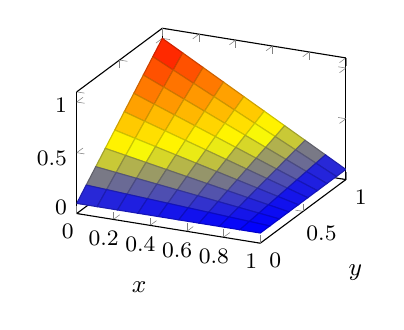
\begin{tikzpicture}
	\begin{axis}[footnotesize,xlabel=$x$,ylabel=$y$,unit vector ratio=]
	\addplot3[surf,samples=10,domain=0:1] {(1-x)*y};
	\end{axis}
\end{tikzpicture}
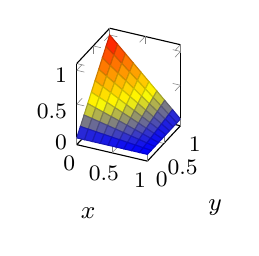
\begin{tikzpicture}
	\begin{axis}[footnotesize,xlabel=$x$,ylabel=$y$,
		unit rescale keep size=false,
		unit vector ratio=1 1 1]
	\addplot3[surf,samples=10,domain=0:1] {(1-x)*y};
	\end{axis}
\end{tikzpicture}
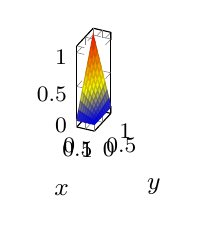
\begin{tikzpicture}
	\begin{axis}[footnotesize,xlabel=$x$,ylabel=$y$,
		unit vector ratio*=0.25 0.5, % the '*' implies 'unit rescale keep size=false'
	]
	\addplot3[surf,samples=10,domain=0:1] {(1-x)*y};
	\end{axis}
\end{tikzpicture}
\end{codeexample}
	\end{pgfplotskeylist}
\end{pgfplotskey}

\begin{pgfplotsxykeylist}{\x\ post scale=\marg{scale} (initially 1)}
	Lets \PGFPlots\ compute the axis scaling based on |width|, |height|, |view|, |plot box ratio|, |axis equal| or explicit unit vectors with |x|, |y|, |z| and \emph{rescales} the resulting vector(s) according to \meta{scale}.
\begin{codeexample}[]
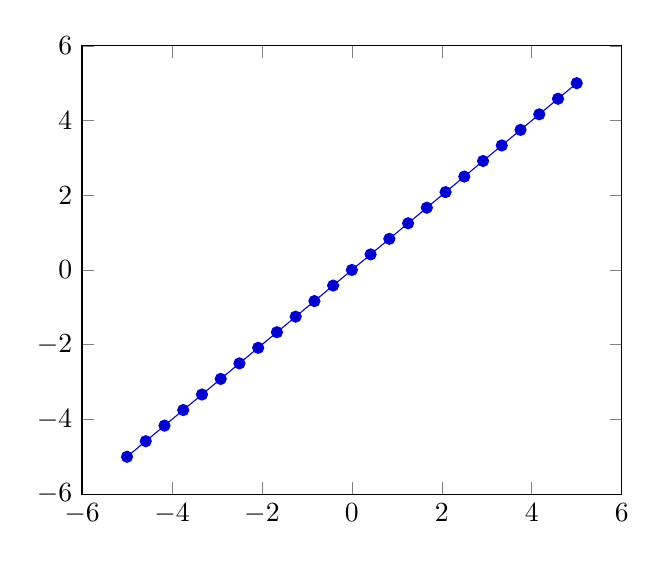
\begin{tikzpicture}
	\begin{axis}[y post scale=1]
	\addplot {x};	
	\end{axis}
\end{tikzpicture}
\begin{tikzpicture}
	\begin{axis}[y post scale=2]
	\addplot {x};	
	\end{axis}
\end{tikzpicture}
\end{codeexample}
	Thus, the axis becomes \emph{larger}. This overrules any previous scaling.

\begin{codeexample}[]
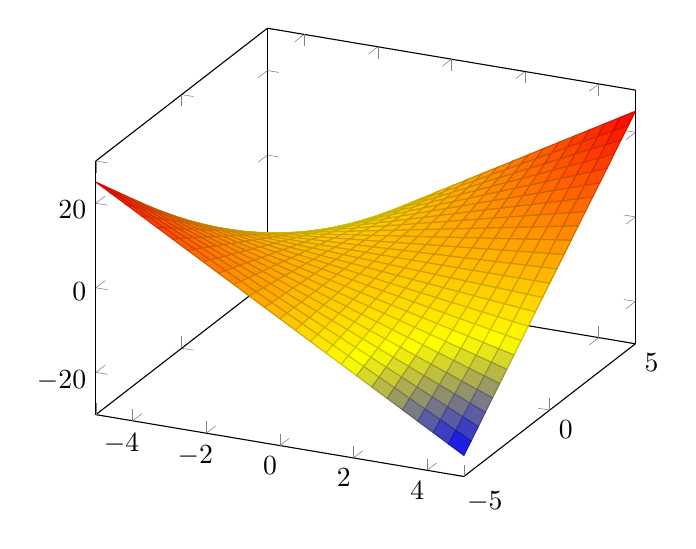
\begin{tikzpicture}
	\begin{axis}[z post scale=1]
		\addplot3[surf] {x*y};
	\end{axis}
\end{tikzpicture}
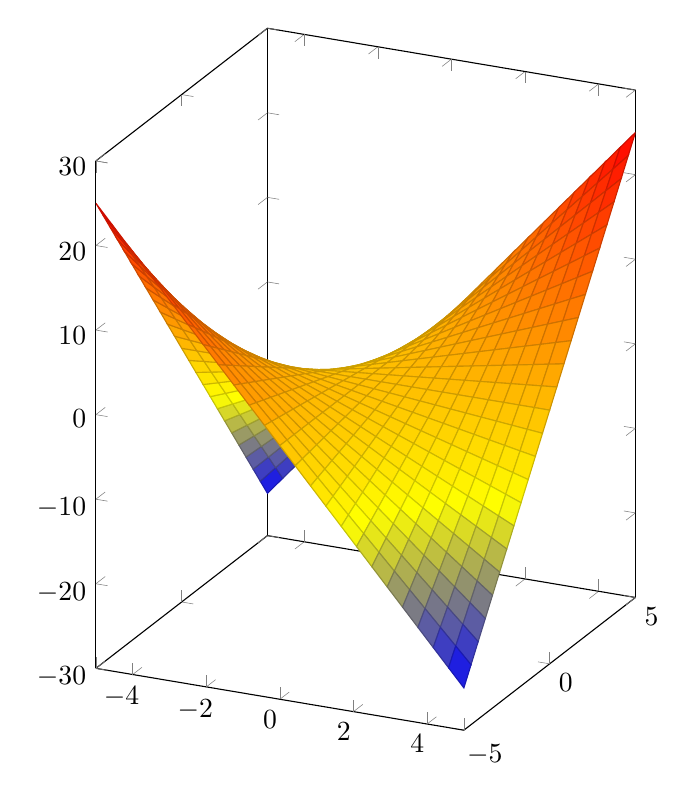
\begin{tikzpicture}
	\begin{axis}[z post scale=2]
		\addplot3[surf] {x*y};
	\end{axis}
\end{tikzpicture}
\end{codeexample}
\end{pgfplotsxykeylist}
